\chapter{داخل الذرة}\label{ch:g9:inside-the-atom}

سنة 1909، في مختبر بمدينة مانشستر، أُطلقت حزمة من جسيمات دقيقة سريعة على
رقاقة من الذهب سُمكها بضع مئات من \omterm{def:g7:atoms-and-molecules:atom}{الذرات}. فاخترق معظمها الرقاقة مباشرة،
كأن الذهب فارغ. لكن جسيمًا واحدًا تقريبًا من كل بضعة آلاف ارتدّ إلى
الوراء. وقال إرنست رذرفورد، الذي أجرى طلابه التجربة: «كان الأمر كأنك
أطلقت قذيفة عيارها خمس عشرة بوصة على ورقة منديل فارتدّت إليك وأصابتك».
\omterm{def:g7:atoms-and-molecules:atom}{فالذرة}، تلك القطعة من المادة التي لا تنقسم، لها بنية --- وهي فارغة كلها
تقريبًا.

\begin{recall}
كل المادة مكوّنة من \omterm{def:g7:atoms-and-molecules:atom}{ذرات}، من نحو مئة نوع مختلف، لكل منها رمز مثل \ce{H}
و\ce{C} و\ce{O} و\ce{Fe}. وتتحد \omterm{def:g7:atoms-and-molecules:atom}{الذرات} في \omterm{def:g7:atoms-and-molecules:molecule}{جزيئات} تصفها صيغ مثل \ce{H2O}
(\cref{ch:g7:atoms-and-molecules}).
\end{recall}

\section{النواة والإلكترونات}

\begin{definition}[النواة والإلكترون]\label{def:g9:inside-the-atom:nucleus}
لكل \omterm{def:g7:atoms-and-molecules:atom}{ذرة} قلب بالغ الصغر وثقيل، هو \emph{النواة}\index{نواة}، يحمل شحنة
كهربائية موجبة. وتتحرك حوله جسيمات أخف منه بكثير، هي
\emph{الإلكترونات}\index{إلكترون}، يحمل كل منها الشحنة السالبة نفسها،
$-e$.
\end{definition}

\begin{proposition}[الذرة متعادلة]\label{prop:g9:inside-the-atom:neutral}
% ledger: const:e
لا تحمل \omterm{def:g7:atoms-and-molecules:atom}{الذرة} في مجموعها أي شحنة كهربائية: فالشحنة الموجبة لنواتها تعادلها
تمامًا الشحنات السالبة لإلكتروناتها. والشحنة $e$ بالغة الصغر:
$e = \qty{1.60e-19}{C}$ (والكولوم، وحدة الشحنة، من شأن كتاب
الفيزياء).
\end{proposition}

\begin{omfigure}
\begin{tikzpicture}[font=\small]
  \shade[inner color=omDef!35, outer color=white] (0,0) circle (2.2);
  \draw[omDef!60, dashed] (0,0) circle (2.2);
  \foreach \a/\r in {20/1.6,95/1.1,150/1.9,215/1.4,290/1.7,340/0.9} {
    \fill[omDef] (\a:\r) circle (0.06);
    \node[font=\scriptsize, omDef] at ($(\a:\r)+(0.18,0.16)$) {$-$};
  }
  \fill[red!70!black] (0,0) circle (0.1);
  \draw[<-, omProp, thick] (-0.12,0.02) -- (-3.0,0.9) node[left, text=black, align=right]
    {النواة: بالغة الصغر،\\ ثقيلة، موجبة};
  \draw[<-, omProp, thick] ($(20:1.6)+(0.08,0.02)$) -- (3.0,0.9) node[right, text=black]
    {إلكترون: خفيف، سالب};
  \draw[<-, omProp, thick] (300:2.2) -- (3.0,-1.4) node[right, text=black, align=left]
    {تتحرك الإلكترونات في سحابة\\ حول النواة};
\end{tikzpicture}

{\small \omterm{def:g7:atoms-and-molecules:atom}{ذرة}، دون مراعاة المقياس. لو رُسمت \omterm{def:g9:inside-the-atom:nucleus}{النواة} بحجم النقطة الحمراء لكان
قطر سحابة \omterm{def:g9:inside-the-atom:nucleus}{الإلكترونات} بضع مئات من الأمتار.}
\end{omfigure}

\section{البروتونات والنيوترونات}

\begin{definition}[البروتون والنيوترون والنوكليون]\label{def:g9:inside-the-atom:proton}
تتكون \omterm{def:g9:inside-the-atom:nucleus}{النواة} من نوعين من الجسيمات: \emph{البروتونات}\index{بروتون}، ويحمل
كل منها الشحنة $+e$، و\emph{النيوترونات}\index{نيوترون}، وهي لا تحمل
شحنة. والبروتونات والنيوترونات، ولها الكتلة نفسها تقريبًا، تسمى معًا
\emph{النوكليونات}\index{نوكليون}.
\end{definition}

\begin{definition}[العدد الذري والعدد الكتلي]\label{def:g9:inside-the-atom:atomic-number}
عدد \omterm{def:g9:inside-the-atom:proton}{البروتونات} في \omterm{def:g9:inside-the-atom:nucleus}{النواة} هو \emph{العدد الذري}\index{عدد ذري}، ويُرمز إليه
بالرمز $Z$. وعدد \omterm{def:g9:inside-the-atom:proton}{النوكليونات} (\omterm{def:g9:inside-the-atom:proton}{البروتونات} \omterm{def:g9:inside-the-atom:proton}{والنيوترونات} معًا) هو
\emph{العدد الكتلي}\index{عدد كتلي}، ويُرمز إليه بالرمز $A$. وعدد
\omterm{def:g9:inside-the-atom:proton}{النيوترونات} هو $N = A - Z$.
\end{definition}

\begin{notation}[رمز النويدة]\label{not:g9:inside-the-atom:symbol}
تُكتب \omterm{def:g7:atoms-and-molecules:atom}{الذرة} ذات \omterm{def:g9:inside-the-atom:nucleus}{النواة} المعيّنة برمزها، مع \omterm{def:g9:inside-the-atom:atomic-number}{العدد الكتلي} في أعلى اليسار
\omterm{def:g9:inside-the-atom:atomic-number}{والعدد الذري} في أسفل اليسار:
\ce{^{A}_{Z}X}. فمثلًا في \ce{^{12}_{6}C} ستة \omterm{def:g9:inside-the-atom:proton}{بروتونات} و$12 - 6 =
6$ \omterm{def:g9:inside-the-atom:proton}{نيوترونات}؛ وفي \ce{^{56}_{26}Fe} ستة وعشرون بروتونًا وثلاثون نيوترونًا.
\end{notation}

\begin{method}[قراءة رمز النويدة]\label{met:g9:inside-the-atom:read}
للرمز \ce{^{A}_{Z}X}:
\begin{enumerate}
  \item \omterm{def:g9:inside-the-atom:proton}{البروتونات}: $Z$؛
  \item \omterm{def:g9:inside-the-atom:proton}{النيوترونات}: $A - Z$؛
  \item \omterm{def:g9:inside-the-atom:nucleus}{إلكترونات} \omterm{def:g7:atoms-and-molecules:atom}{الذرة} المتعادلة: $Z$، أي عدد \omterm{def:g9:inside-the-atom:proton}{البروتونات} نفسه.
\end{enumerate}
وللرمز \ce{^{23}_{11}Na}: 11 بروتونًا، و12 نيوترونًا، و11 إلكترونًا.
\end{method}

\begin{omfigure}
\begin{tikzpicture}[font=\small]
  \node[font=\Huge, inner sep=1pt] (x) at (0,0) {\ce{^{35}_{17}Cl}};
  \draw[<-, omProp, thick, shorten <=3pt] ([xshift=5pt,yshift=-7pt]x.north west) -- (-2.6,1.0)
    node[left, text=black, align=right] {\foreignlanguage{arabic}{العدد الكتلي $A = 35$:}\\ البروتونات + النيوترونات};
  \draw[<-, omProp, thick, shorten <=3pt] ([xshift=5pt,yshift=7pt]x.south west) -- (-2.6,-1.0)
    node[left, text=black, align=right] {\foreignlanguage{arabic}{العدد الذري $Z = 17$:}\\ البروتونات};
  \draw[<-, omProp, thick] ([xshift=2pt]x.east) -- (2.2,0) node[right, text=black,
    align=left] {رمز العنصر:\\ الكلور};
\end{tikzpicture}

{\small قراءة رمز النويدة: في \omterm{def:g7:atoms-and-molecules:atom}{ذرة} الكلور هذه 17 بروتونًا، و$35 - 17 = 18$
نيوترونًا، و17 إلكترونًا حين تكون متعادلة.}
\end{omfigure}

\section{العنصر الكيميائي ونظائره}

\begin{definition}[العنصر الكيميائي]\label{def:g9:inside-the-atom:element}
\emph{العنصر الكيميائي}\index{عنصر كيميائي} مجموعة كل \omterm{def:g7:atoms-and-molecules:atom}{الذرات}، وكل \omterm{def:g7:atoms-and-molecules:atom}{الذرات}
المشحونة المشتقة منها، التي لها \omterm{def:g9:inside-the-atom:atomic-number}{العدد الذري} $Z$ نفسه. ولكل عنصر اسم
ورمز: فكل \omterm{def:g7:atoms-and-molecules:atom}{ذرة} فيها 6 \omterm{def:g9:inside-the-atom:proton}{بروتونات} \omterm{def:g7:atoms-and-molecules:atom}{ذرة} كربون، \ce{C}؛ وكل \omterm{def:g7:atoms-and-molecules:atom}{ذرة} فيها 8
\omterm{def:g9:inside-the-atom:proton}{بروتونات} \omterm{def:g7:atoms-and-molecules:atom}{ذرة} أكسجين، \ce{O}.
\end{definition}

\begin{definition}[النظائر]\label{def:g9:inside-the-atom:isotope}
\omterm{def:g7:atoms-and-molecules:atom}{ذرات} العنصر الواحد التي تختلف في عدد نيوتروناتها، ومن ثم في عددها الكتلي،
هي \emph{نظائر}\index{نظير} ذلك العنصر. فلها $Z$ نفسه و$A$
مختلف.
\end{definition}

\begin{example}[نظائر الكربون والهيدروجين]\label{ex:g9:inside-the-atom:isotopes}
% ledger: iso:C12, iso:C13, iso:H2
الكربون الطبيعي نحو \qty{98.9}{\percent} منه كربون 12، \ce{^{12}_{6}C}،
و\qty{1.1}{\percent} كربون 13، \ce{^{13}_{6}C}، ومعهما أثر من
الكربون 14، \ce{^{14}_{6}C}، الذي يُستعمل تحوّله البطيء إلى \omterm{def:g9:inside-the-atom:nucleus}{نواة} أخرى
لتأريخ الأخشاب والعظام القديمة (والنشاط الإشعاعي من شأن كتاب الفيزياء).
وللهيدروجين ثلاثة \omterm{def:g9:inside-the-atom:isotope}{نظائر}: \ce{^{1}_{1}H}، بلا أي \omterm{def:g9:inside-the-atom:proton}{نيوترون}، وهو الأشيع بفارق
كبير؛ والدوتيريوم \ce{^{2}_{1}H}، بضع \omterm{def:g7:atoms-and-molecules:atom}{ذرات} في كل مئة ألف؛ والتريتيوم
\ce{^{3}_{1}H}.
\end{example}

\begin{proposition}[النظائر تتشابه في سلوكها الكيميائي]\label{prop:g9:inside-the-atom:alike}
كيمياء \omterm{def:g7:atoms-and-molecules:atom}{الذرة} تتوقف على إلكتروناتها، ولنظائر العنصر الواحد العدد نفسه من
\omterm{def:g9:inside-the-atom:nucleus}{الإلكترونات}. ولذلك تتفاعل \omterm{def:g9:inside-the-atom:isotope}{النظائر} بالطريقة نفسها: فالماء المصنوع بالدوتيريوم
يشبه الماء العادي مظهرًا وسلوكًا شبهًا شبه تام.
\end{proposition}

\begin{omfigure}
\begin{tikzpicture}[font=\small, p/.style={circle, inner sep=0pt, minimum size=4.2mm,
    ball color=red!65}, n/.style={circle, inner sep=0pt, minimum size=4.2mm,
    ball color=black!20}]
  \node[p] at (0,0) {};
  \node[anchor=north, align=center] at (0,-0.45) {\ce{^{1}_{1}H}\\ \foreignlanguage{arabic}{\babelsublr{1} بروتون}};
  \node[p] at (3.0,0) {}; \node[n] at (3.35,0.1) {};
  \node[anchor=north, align=center] at (3.2,-0.45) {\ce{^{2}_{1}H}\\ \foreignlanguage{arabic}{\babelsublr{1} بروتون، \babelsublr{1} نيوترون}};
  \node[p] at (6.4,0) {}; \node[n] at (6.75,0.12) {}; \node[n] at (6.55,0.35) {};
  \node[anchor=north, align=center] at (6.6,-0.45) {\ce{^{3}_{1}H}\\ \foreignlanguage{arabic}{\babelsublr{1} بروتون، \babelsublr{2} نيوترون}};
  \node[draw=black!30, fill=red!65, circle, minimum size=3mm, inner sep=0pt] at (9.1,0.2) {};
  \node[anchor=west] at (9.3,0.2) {بروتون};
  \node[draw=black!30, fill=black!20, circle, minimum size=3mm, inner sep=0pt] at (9.1,-0.3) {};
  \node[anchor=west] at (9.3,-0.3) {نيوترون};
\end{tikzpicture}

{\small أنوية \omterm{def:g9:inside-the-atom:isotope}{نظائر} الهيدروجين الثلاثة: \omterm{def:g9:inside-the-atom:proton}{بروتون} واحد في كل منها، و0 أو 1
أو 2 \omterm{def:g9:inside-the-atom:proton}{نيوترون}.}
\end{omfigure}

\section{الأحجام والكتل}

\begin{proposition}[النواة بالغة الصغر وتحمل كل الكتلة تقريبًا]\label{prop:g9:inside-the-atom:sizes}
% ledger: const:a0, r:proton, const:mp, const:mn, const:me
قطر \omterm{def:g7:atoms-and-molecules:atom}{الذرة} نحو \qty{e-10}{m}؛ وقطر نواتها من \qty{e-15}{m} إلى
\qty{e-14}{m} تقريبًا: أي أصغر منها بنحو عشرة آلاف إلى مئة ألف مرة.
وكتل الجسيمات هي
\[
  m_p = \qty{1.673e-27}{kg},\qquad m_n = \qty{1.675e-27}{kg},\qquad
  m_e = \qty{9.11e-31}{kg}.
\]
\omterm{def:g9:inside-the-atom:proton}{فالبروتون} أثقل من \omterm{def:g9:inside-the-atom:nucleus}{الإلكترون} بنحو 1836 مرة، ولذلك فإن أكثر من
\qty{99.9}{\percent} من كتلة \omterm{def:g7:atoms-and-molecules:atom}{الذرة} في نواتها.
\end{proposition}

\begin{example}[كرة زجاجية في ملعب]\label{ex:g9:inside-the-atom:marble}
لو كانت \omterm{def:g9:inside-the-atom:nucleus}{نواة} \omterm{def:g7:atoms-and-molecules:atom}{الذرة} كرة زجاجية صغيرة قطرها \qty{1}{cm} لكان قطر \omterm{def:g7:atoms-and-molecules:atom}{الذرة} نحو
$\qty{1}{cm} \times 100\,000 = \qty{1}{km}$: كرة صغيرة في وسط ملعب ضخم،
وبضع \omterm{def:g7:atoms-and-molecules:atom}{ذرات} من الغبار --- هي \omterm{def:g9:inside-the-atom:nucleus}{الإلكترونات} --- تدور حول المدرجات. فالمادة في
معظمها فراغ.
\end{example}

\begin{method}[كتلة الذرة]\label{met:g9:inside-the-atom:mass}
بما أن \omterm{def:g9:inside-the-atom:proton}{للبروتونات} \omterm{def:g9:inside-the-atom:proton}{والنيوترونات} الكتلة نفسها تقريبًا وأن \omterm{def:g9:inside-the-atom:nucleus}{الإلكترونات} خفيفة
جدًا، فإن كتلة \omterm{def:g7:atoms-and-molecules:atom}{الذرة} قريبة من $A \times
\qty{1.67e-27}{kg}$، حيث $A$ عددها الكتلي. \omterm{def:g7:atoms-and-molecules:atom}{ذرة} كربون 12:
$12 \times 1.67 \times 10^{-27} = \qty{2.00e-26}{kg}$.
\end{method}

\section{تاريخ موجز لنموذج الذرة}

\begin{history}[من الذرة التي لا تنقسم إلى النواة، 1897--1932]
اكتشف ج.~ج.~طومسون \omterm{def:g9:inside-the-atom:nucleus}{الإلكترون} سنة 1897، وهو جسيم أخف بكثير من أي \omterm{def:g7:atoms-and-molecules:atom}{ذرة}:
\omterm{def:g7:atoms-and-molecules:atom}{فالذرات} تنقسم إذن. وتصوّر \omterm{def:g7:atoms-and-molecules:atom}{الذرة} كرة من مادة موجبة تتخللها \omterm{def:g9:inside-the-atom:nucleus}{الإلكترونات}. وفي
1909--1911 بيّنت تجربة رقاقة الذهب التي أجراها فريق رذرفورد أن الشحنة
الموجبة وكل الكتلة تقريبًا مستقرة في \omterm{def:g9:inside-the-atom:nucleus}{نواة} بالغة الصغر. وفي 1913 اقترح نيلز
بور أن \omterm{def:g9:inside-the-atom:nucleus}{الإلكترونات} تشغل مستويات طاقة محددة حولها، وفي 1932 اكتشف جيمس
تشادويك \omterm{def:g9:inside-the-atom:proton}{النيوترون}.
\end{history}

\begin{omfigure}
\begin{minipage}[b]{0.3\linewidth}\centering
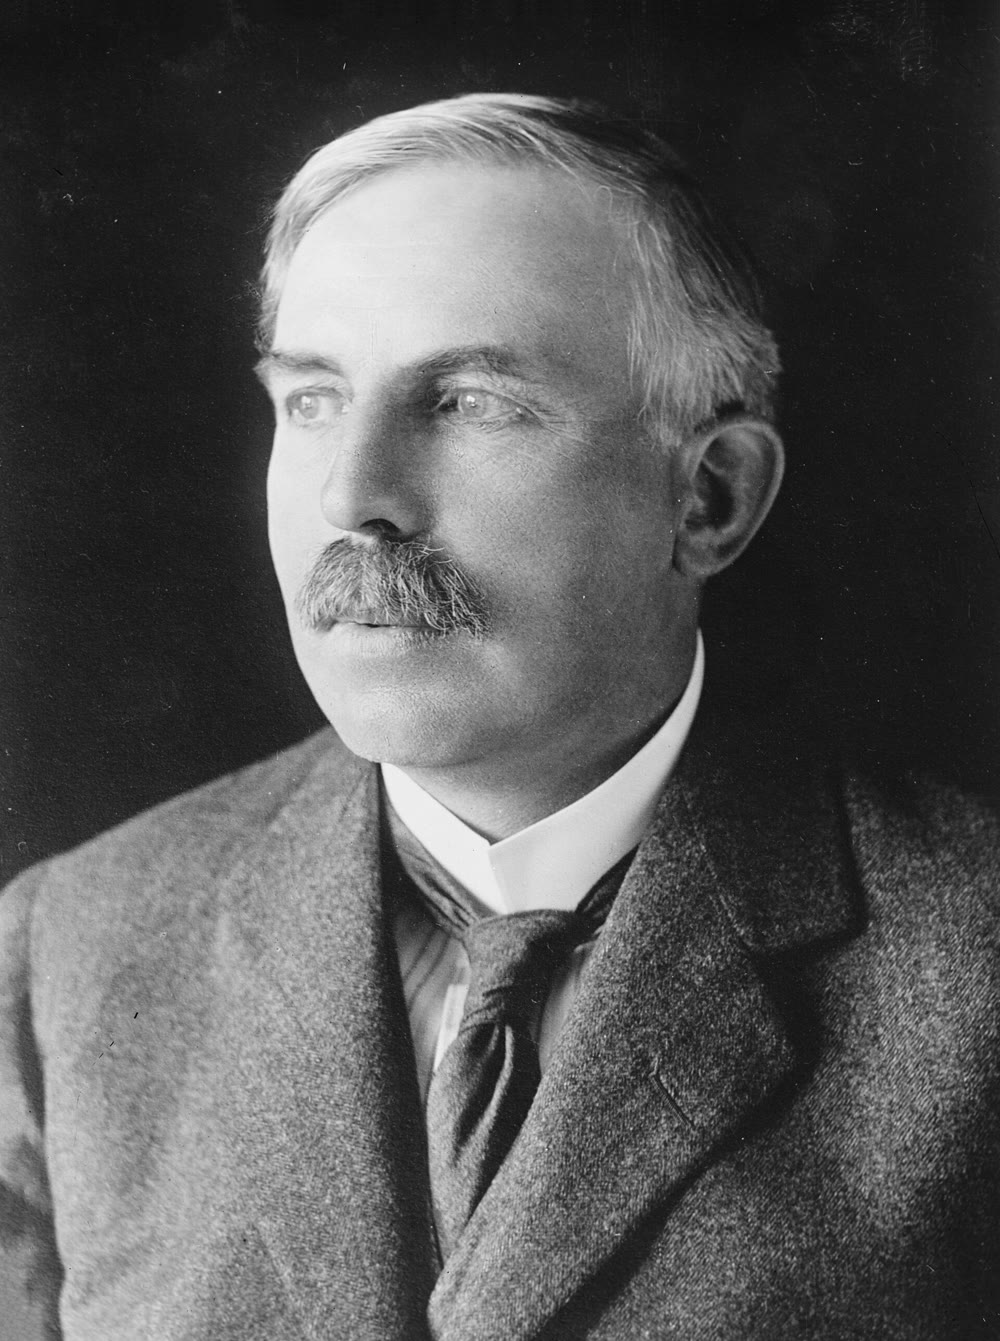
\includegraphics[width=\linewidth]{images/book1/rutherford.jpg}

{\small إرنست رذرفورد (1871--1937).}
\end{minipage}\hfill
\begin{minipage}[b]{0.66\linewidth}\centering
\begin{tikzpicture}[font=\small]
  \fill[black!45] (0,-0.5) rectangle (0.9,0.5);
  \node[anchor=north, align=center] at (0.45,-0.55) {مصدر\\ جسيمات ألفا};
  \draw[->, thick, red!70!black] (0.9,0) -- (2.8,0);
  \fill[yellow!70!orange] (2.8,-1.6) rectangle (2.88,1.6);
  \node[anchor=north] at (2.84,-1.65) {رقاقة الذهب};
  \draw[omDef!40, line width=4pt] (5.6,-1.8) arc[start angle=-30, end angle=30, radius=3.6];
  \foreach \y in {-0.3,-0.1,0.1,0.3} \draw[->, red!70!black] (2.88,\y) -- (5.3,\y);
  \draw[->, red!70!black] (2.88,0.05) -- (5.0,1.15);
  \draw[->, red!70!black] (2.88,-0.05) -- (4.9,-1.3);
  \draw[->, red!70!black, thick] (2.8,0.02) .. controls (2.2,0.35) .. (1.6,0.95);
  \node[anchor=west, align=left, font=\footnotesize] at (6.25,0) {معظمها\\ يمر\\ مباشرة};
  \node[anchor=south, align=center, font=\footnotesize] at (1.6,1.0) {قليل جدًا\\ يرتد};
\end{tikzpicture}

{\small تجربة رقاقة الذهب: تمر معظم الجسيمات مباشرة؛ وينحرف بعضها؛
ويرتد قليل جدًا منها عن \omterm{def:g9:inside-the-atom:nucleus}{نواة}.}
\end{minipage}
\end{omfigure}

\section{تمارين}

\begin{exercise}[$\star$]\label{exo:g9:inside-the-atom:1}
سمِّ جسيمات \omterm{def:g9:inside-the-atom:nucleus}{النواة} والجسيمات التي حولها، مع إشارة
شحنتها.
\end{exercise}

\begin{exercise}[$\star$]\label{exo:g9:inside-the-atom:2}
أعطِ عدد \omterm{def:g9:inside-the-atom:proton}{البروتونات} \omterm{def:g9:inside-the-atom:proton}{والنيوترونات} \omterm{def:g9:inside-the-atom:nucleus}{والإلكترونات} في \ce{^{16}_{8}O}
و\ce{^{27}_{13}Al} و\ce{^{40}_{20}Ca}.
\end{exercise}

\begin{exercise}[$\star$]\label{exo:g9:inside-the-atom:3}
لماذا تكون \omterm{def:g7:atoms-and-molecules:atom}{الذرة} متعادلة كهربائيًا؟
\end{exercise}

\begin{exercise}[$\star$]\label{exo:g9:inside-the-atom:4}
في \omterm{def:g7:atoms-and-molecules:atom}{ذرة} 26 بروتونًا و30 نيوترونًا. اكتب رمز نويدتها (والعنصر هو الحديد،
\ce{Fe}).
\end{exercise}

\begin{exercise}[$\star\star$]\label{exo:g9:inside-the-atom:5}
هل \ce{^{35}_{17}Cl} و\ce{^{37}_{17}Cl} العنصر نفسه؟ وهل هما
نظيران؟ علّل.
\end{exercise}

\begin{exercise}[$\star\star$]\label{exo:g9:inside-the-atom:6}
هل \ce{^{14}_{6}C} و\ce{^{14}_{7}N} نظيران؟ علّل.
\end{exercise}

\begin{exercise}[$\star\star$]\label{exo:g9:inside-the-atom:7}
احسب، بالكتابة العلمية، الكتلة التقريبية \omterm{def:g7:atoms-and-molecules:atom}{لذرة}
\ce{^{56}_{26}Fe}.
\end{exercise}

\begin{exercise}[$\star\star$]\label{exo:g9:inside-the-atom:8}
في تجربة رقاقة الذهب، لماذا تمر معظم الجسيمات مباشرة عبر
الذهب؟
\end{exercise}

\begin{exercise}[$\star\star$]\label{exo:g9:inside-the-atom:9}
كم مرة تصغر \omterm{def:g9:inside-the-atom:nucleus}{نواة} قطرها \qty{e-15}{m} عن \omterm{def:g7:atoms-and-molecules:atom}{ذرة} قطرها
\qty{e-10}{m}؟ اكتب الجواب قوةً للعدد عشرة.
\end{exercise}

\begin{exercise}[$\star\star$]\label{exo:g9:inside-the-atom:10}
لماذا يكون \omterm{def:g9:inside-the-atom:isotope}{لنظائر} العنصر الواحد السلوك الكيميائي نفسه؟
\end{exercise}

\begin{exercise}[$\star\star\star$]\label{exo:g9:inside-the-atom:11}
في \omterm{def:g7:atoms-and-molecules:atom}{ذرة} الحديد 26 إلكترونًا. احسب كتلتها الكلية، ثم الكسر الذي تمثله من
كتلة \omterm{def:g7:atoms-and-molecules:atom}{ذرة} \ce{^{56}_{26}Fe} (استعمل الكتلة التي وجدتها في
التمرين~7).
\end{exercise}

\begin{exercise}[$\star\star\star$]\label{exo:g9:inside-the-atom:12}
% ledger: iso:Cu63, iso:Cu65
النحاس الطبيعي \qty{69.15}{\percent} منه نحاس 63 و\qty{30.85}{\percent}
نحاس 65. من بين 10\,000 \omterm{def:g7:atoms-and-molecules:atom}{ذرة} نحاس، كم \omterm{def:g7:atoms-and-molecules:atom}{ذرة} من كل \omterm{def:g9:inside-the-atom:isotope}{نظير}؟
وما متوسط عدد \omterm{def:g9:inside-the-atom:proton}{النوكليونات} في \omterm{def:g7:atoms-and-molecules:atom}{ذرة} النحاس؟
\end{exercise}

\clearpage % keeps the heading with its problem box (it was stranded at a page foot)
\section{مسألة: وزن الكلور}

\begin{problem}[{مسألة نهاية الأسبوع --- نظيرا الكلور، وكتلة كل ذرة،
ومتوسط كتلة ذرة الكلور}]
\label{pb:g9:inside-the-atom:1}
% ledger: iso:Cl35, iso:Cl37, const:me, const:mp, const:mn
الكلور الطبيعي \omterm{def:g6:pure-substances-and-mixtures:mixture}{خليط} من نظيرين، الكلور 35 والكلور 37: فمن كل 1000 \omterm{def:g7:atoms-and-molecules:atom}{ذرة}
كلور، نحو 758 كلور 35 و242 كلور 37. خذ كتلة \omterm{def:g9:inside-the-atom:proton}{النوكليون}
\qty{1.67e-27}{kg} وكتلة \omterm{def:g9:inside-the-atom:nucleus}{الإلكترون} \qty{9.11e-31}{kg}. \omterm{def:g9:inside-the-atom:atomic-number}{والعدد الذري}
للكلور 17.

\medskip
\noindent\textbf{الجزء الأول --- نواتان.}
\begin{enumerate}
  \item اكتب رمزي نويدتي النظيرين.
  \item أعطِ عدد \omterm{def:g9:inside-the-atom:proton}{البروتونات} \omterm{def:g9:inside-the-atom:proton}{والنيوترونات} \omterm{def:g9:inside-the-atom:nucleus}{والإلكترونات} في كل منهما.
  \item لماذا يسمى كلاهما كلورًا؟ ولماذا هما نظيران؟
  \item هل تتفاعل عيّنة من الكلور 37 مع الصوديوم بالطريقة نفسها التي تتفاعل
        بها عيّنة من الكلور 35؟ علّل.
\end{enumerate}

\medskip
\noindent\textbf{الجزء الثاني --- كتلة كل \omterm{def:g7:atoms-and-molecules:atom}{ذرة}.}
\begin{enumerate}[resume]
  \item احسب كتلة \omterm{def:g9:inside-the-atom:nucleus}{نواة} \omterm{def:g7:atoms-and-molecules:atom}{ذرة} الكلور 35.
  \item احسب كتلة \omterm{def:g9:inside-the-atom:nucleus}{الإلكترونات} السبعة عشر، وتحقق من أنه يمكن إهمالها إلى جانب
        \omterm{def:g9:inside-the-atom:nucleus}{النواة}.
  \item احسب كتلة \omterm{def:g7:atoms-and-molecules:atom}{ذرة} الكلور 37.
  \item كم \omterm{def:g7:atoms-and-molecules:atom}{ذرة} من الكلور 35 تزن \qty{1}{g}؟ أعطِ الجواب
        بالكتابة العلمية.
\end{enumerate}

\medskip
\noindent\textbf{الجزء الثالث --- \omterm{def:g7:atoms-and-molecules:atom}{الذرة} المتوسطة.}
\begin{enumerate}[resume]
  \item ما النسبة المئوية \omterm{def:g7:atoms-and-molecules:atom}{لذرات} الكلور 35 بين \omterm{def:g7:atoms-and-molecules:atom}{ذرات} الكلور؟ ولذرات الكلور 37؟
  \item في 1000 \omterm{def:g7:atoms-and-molecules:atom}{ذرة} من الكلور الطبيعي، احسب الكتلة الكلية \omterm{def:g7:atoms-and-molecules:atom}{لذرات} الكلور 35
        ولذرات الكلور 37.
  \item احسب كتلة هذه \omterm{def:g7:atoms-and-molecules:atom}{الذرات} الألف.
  \item استنتج متوسط كتلة \omterm{def:g7:atoms-and-molecules:atom}{ذرة} الكلور.
\end{enumerate}
\end{problem}
